\documentclass[11pt,a4paper,twoside,openright]{report}

\usepackage{graphicx}
\graphicspath{ {./images/} }
\usepackage[top=25mm,bottom=25mm,right=25mm,left=30mm,head=12.5mm,foot=12.5mm]{geometry}
\let\openright=\cleardoublepage

\usepackage[a-2u]{pdfx}

\usepackage[
   backend=biber
%  ,style=iso-authoryear
  ,style=alphabetic
  ,citestyle=numeric
  ,sortlocale=cs_CZ
  ,bibencoding=UTF8
  %,block=ragged
]{biblatex}
\addbibresource{references.bib}

%% Přepneme na českou sazbu, fonty Latin Modern a kódování češtiny
\usepackage[czech]{babel}
\usepackage{lmodern}
\usepackage[T1]{fontenc}
\usepackage{textcomp}
\usepackage[utf8]{inputenc}

% Set fonts
\RequirePackage[osf]{mathpazo} % Palatino with oldstyle figures
\newcommand\liningnums[1]{\fontfamily{ppl}\selectfont#1}
\RequirePackage{eulervm}
\RequirePackage[scaled=.8819]{sourcecodepro} % Source Code Pro typeface for monospace

%%% Další užitečné balíčky (jsou součástí běžných distribucí LaTeXu)
\usepackage{amsmath}        % rozšíření pro sazbu matematiky
\usepackage{amsfonts}       % matematické fonty
\usepackage{amsthm}         % sazba vět, definic apod.
\usepackage{bm}             % tučné symboly (příkaz \bm)
\usepackage{graphicx}       % vkládání obrázků
\usepackage{fancyvrb}       % vylepšené prostředí pro strojové písmo
\usepackage{fancyhdr}       % prostředí pohodlnější nastavení hlavy a paty stránek
\usepackage{icomma}         % inteligetní čárka v matematickém módu
\usepackage{dcolumn}        % lepší zarovnání sloupců v tabulkách
\usepackage{booktabs}       % lepší vodorovné linky v tabulkách
\makeatletter
\@ifpackageloaded{xcolor}{
   \@ifpackagewith{xcolor}{usenames}{}{\PassOptionsToPackage{usenames}{xcolor}}
  }{\usepackage[usenames]{xcolor}} % barevná sazba
\makeatother
\usepackage{multicol}       % práce s více sloupci na stránce
\usepackage{caption}
\usepackage{enumitem}
\usepackage{lipsum}
\setlist[itemize]{noitemsep, topsep=0pt, partopsep=0pt}
\setlist[enumerate]{noitemsep, topsep=0pt, partopsep=0pt}
\setlist[description]{noitemsep, topsep=0pt, partopsep=0pt}
\usepackage{pdfpages}

\usepackage{tocloft}
\setlength\cftparskip{0pt}
\setlength\cftbeforechapskip{1.5ex}
\setlength\cftfigindent{0pt}
\setlength\cfttabindent{0pt}
\setlength\cftbeforeloftitleskip{0pt}
\setlength\cftbeforelottitleskip{0pt}
\setlength\cftbeforetoctitleskip{0pt}
\renewcommand{\cftlottitlefont}{\Huge\bfseries}
\renewcommand{\cftloftitlefont}{\Huge\bfseries}
\renewcommand{\cfttoctitlefont}{\Huge\bfseries}

% vyznaceni odstavcu
\parindent=0pt
\parskip=11pt

% zakaz vdov a sirotku - jednoradkovych pocatku ci koncu odstavcu na prechodu mezi strankami
\clubpenalty=1000
\widowpenalty=1000
\displaywidowpenalty=1000

% nastaveni radkovani
\renewcommand{\baselinestretch}{1.20}

% nastavení hlavy a paty stránek
\fancyhf{}
\renewcommand{\chaptermark}[1]{\markboth{#1}{}}
\fancyhead[RO,LE]{\leftmark}
\fancyfoot[RO,LE]{\thepage}
%\renewcommand{\footrulewidth}{0pt}
\fancypagestyle{plain}{%
\fancyhf{} % clear all header and footer fields
\fancyfoot[RO,LE]{\thepage}
\renewcommand{\headrulewidth}{0pt}
%\renewcommand{\footrulewidth}{0.5pt}
}

% Tato makra přesvědčují mírně ošklivým trikem LaTeX, aby hlavičky kapitol
% sázel příčetněji a nevynechával nad nimi spoustu místa. Směle ignorujte.
\makeatletter
\def\@makechapterhead#1{
  {\parindent \z@ \raggedright 
   \Huge\bfseries \thechapter. #1
   \par\nobreak
   \vskip 20\p@
}}
\def\@makeschapterhead#1{
  {\parindent \z@ \raggedright 
   \Huge\bfseries #1
   \par\nobreak
   \vskip 20\p@
}}
\makeatother

% Trochu volnější nastavení dělení slov, než je default.
\lefthyphenmin=2
\righthyphenmin=2

% Zapne černé "slimáky" na koncích řádků, které přetekly, abychom si
% jich lépe všimli.
\overfullrule=1mm

%% Balíček hyperref, kterým jdou vyrábět klikací odkazy v PDF,
%% ale hlavně ho používáme k uložení metadat do PDF (včetně obsahu).
%% Většinu nastavítek přednastaví balíček pdfx.
\hypersetup{unicode}
\hypersetup{breaklinks=true}
\hypersetup{hidelinks}

%%% Prostředí pro sazbu kódu, případně vstupu/výstupu počítačových
%%% programů. (Vyžaduje balíček fancyvrb -- fancy verbatim.)

\DefineVerbatimEnvironment{code}{Verbatim}{fontsize=\small, frame=single}



\def\NazevPrace{Webová aplikace na anonymní zpětnou vazbu z výuky}
\def\Trida{4.A}
\def\AutorPrace{Matyáš Neruda}
\def\DatumOdevzdani{3.3.2024}

% Vedoucí práce: Jméno a příjmení s~tituly
\def\Vedouci{Šimon Schierreich}

% Studijní program a obor
\def\StudijniProgram{studijní program}
\def\StudijniObor{7941K41 Čtyřleté gymnázium pro absolventy ZŠ}

% Text čestného prohlášení
\def\Prohlaseni{Prohlašuji, že jsem svou práci vypracoval samostatně a použil jsem pouze prameny a literaturu
uvedené v~seznamu bibliografických záznamů. Nemám žádné námitky proti zpřístupňování této práce v~souladu se
zákonem č. 121/2000 Sb. o~právu autorském, o~právech souvisejících s~právem autorským a
o~změně některých zákonů (autorský zákon) ve znění pozdějších předpisů.}

% Text poděkování
\def\Podekovani{%
Vážení rodiče. Chtěl bych vám touto cestou vyjádřit upřímné poděkování za veškerou podporu, kterou jste mi poskytovali během mého studia. Vaše trpělivost, povzbuzování a neustálá motivace hrály klíčovou roli v mém vzdělávacím procesu a já si toho velice vážím. Panu učiteli Schierreichovi děkuji za jeho čas a dobré rady při konzultaci maturitní práce.
}

% Abstrakt česky
\def\Abstrakt{%
Maturitní práce se zaměřuje na vývoj webové aplikace na anonymní zpětnou vazbu z výuky.
V první, teoretické části, je podrobně popsán význam funkcí aplikace pro jednotlivé role uživatelů.
Druhá část se věnuje popisu backendu aplikace. Zde je popsána manipulace s daty v Pythonu s využitím frameworku Flask. Jsou zde detailně popsány použité routy a dotazy potřebné pro práci s databází, stejně jako návrh tabulek v databázi.
Ve frontendové části práce je popsána tvorba základní struktury stránek pomocí HTML a šablonovacího jazyka Jinja. Dále je zde popsána implementace interaktivních prvků a stylování pomocí JavaScriptu, CSS a frameworku Bootstrap.
}

% Abstrakt anglicky
\def\AbstraktEN{%
The graduation thesis focuses on the development of a web application to anonymous feedback from teaching. The first, theoretical part, details the importance of the functions of the application for individual user roles.
The second part is devoted to describing the backend of the application. This describes the manipulation of data in Python using the Flask framework. There are detailed descriptions of the used rushes and queries needed to work with the database, as well as the design of the tables in the database.
The frontend part of the work describes the creation of the basic page structure using HTML and the Jinja template language. It also describes the implementation of interactive elements and styling using JavaScript, CSS and the Bootstrap framework.
}

% 3 až 5 klíčových slov
\def\KlicovaSlova{HTML, SQL, Python, Flask, Bootstrap, Jinja, Web, Aplikace, Student, Učitel}
% 3 až 5 klíčových slov anglicky
\def\KlicovaSlovaEN{HTML, SQL, Python, Flask, Bootstrap, Jinja, Web, Application, Student, Teacher}


\begin{document}

%%% Titulní strana práce a další povinné informační strany

%%% Titulní strana práce

\pagestyle{empty}
\pagenumbering{gobble}
\hypersetup{pageanchor=false}

\begin{center}
\LARGE
\textbf{GYMNASIUM JANA KEPLERA}\\
{\large Parléřova 2/118, 169 00 Praha 6}

\vspace{\stretch{3}}


\includegraphics[width=.3\textwidth]{img/logo}

\vspace{\stretch{3}}

{\Huge\bfseries\NazevPrace}

\vspace{8mm}
\mdseries{Maturitní práce}

\vspace{\stretch{8}}
\large
\begin{tabular}{rl}
Autor: & \AutorPrace \\
\noalign{\vspace{2mm}}
Třída: & \Trida\\
\noalign{\vspace{2mm}}
Školní rok: & 2020/2021\\
\noalign{\vspace{2mm}}
Předmět: & Informatika \\
\noalign{\vspace{2mm}}
Vedoucí práce: & \Vedouci \\
\end{tabular}

\vspace{20mm}
Praha, \DatumOdevzdani
\end{center}


\openright

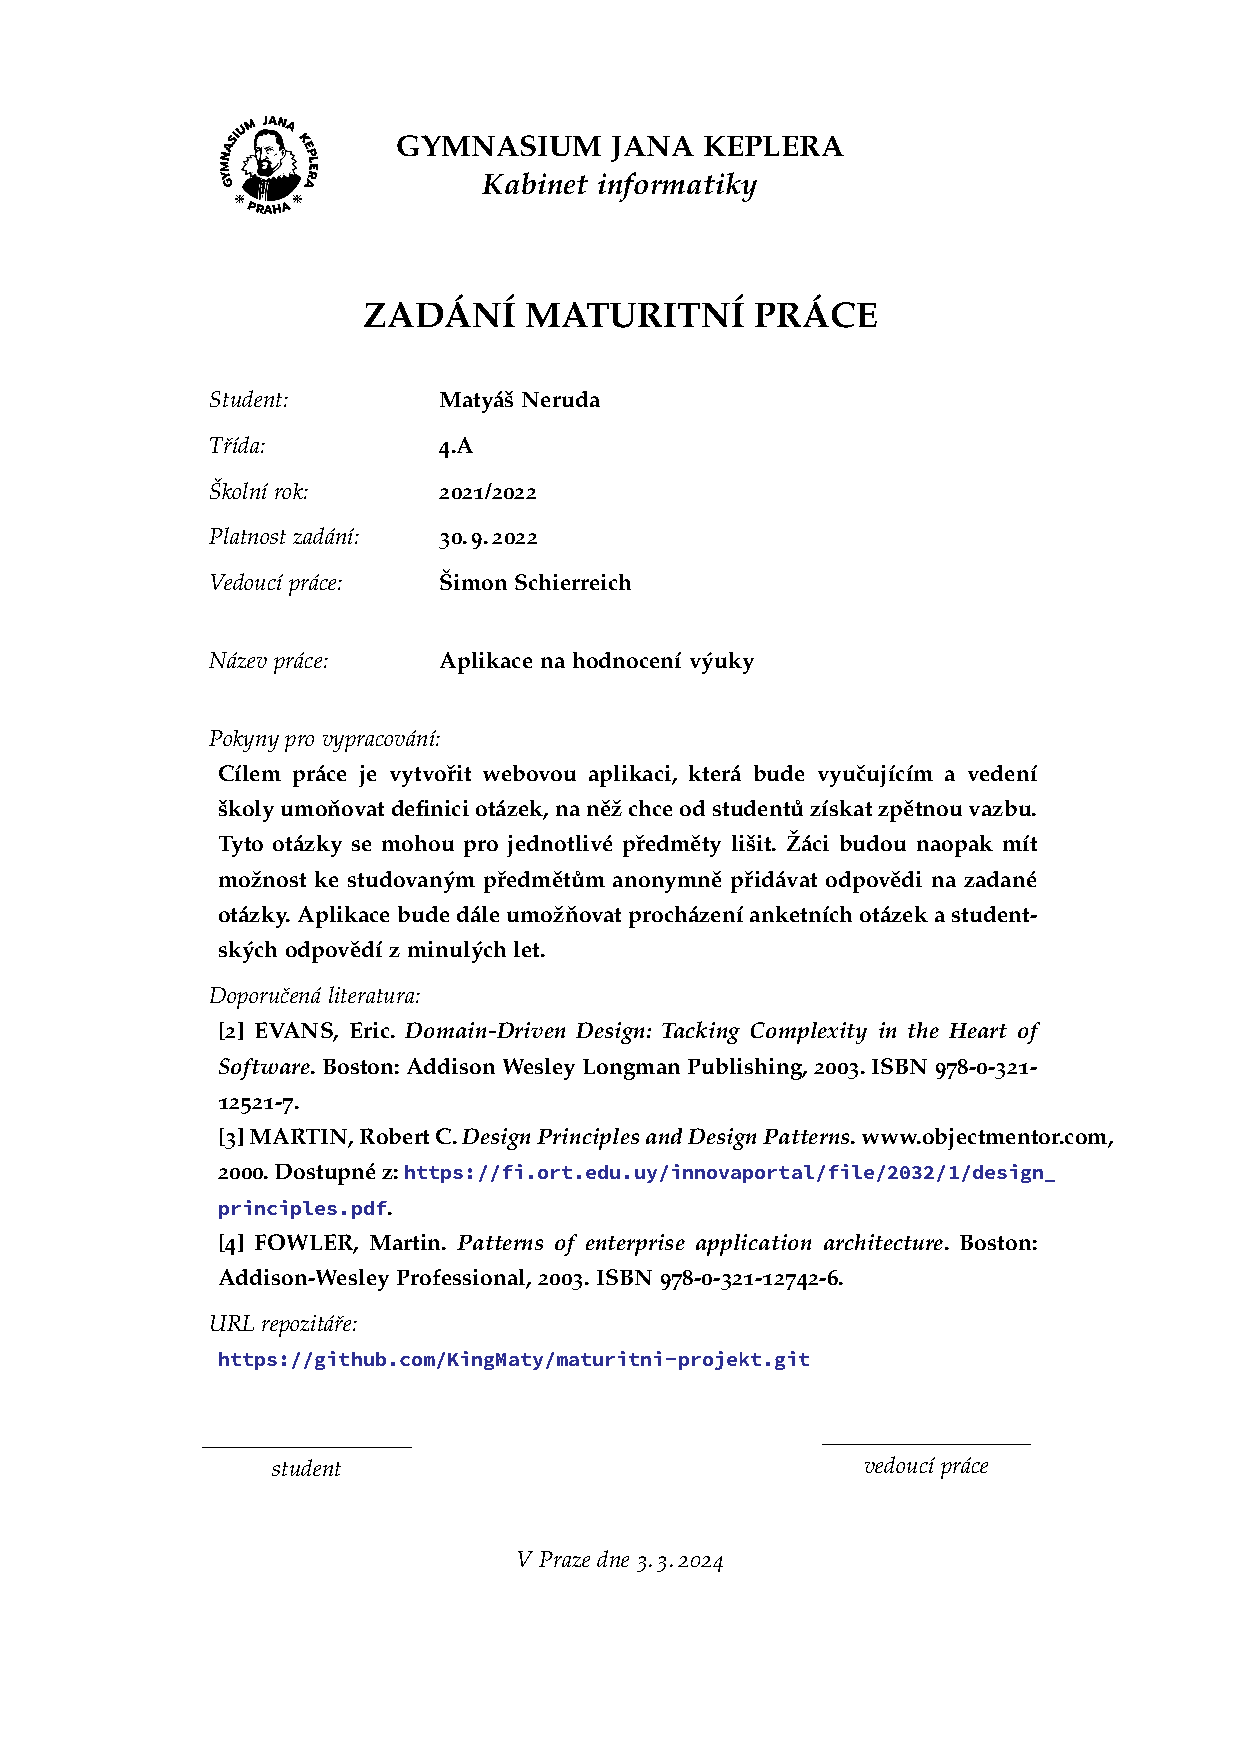
\includepdf[]{zadani.pdf}


%%% Strana s čestným prohlášením k bakalářské práci

\hypersetup{pageanchor=true}
\cleardoublepage
\vspace*{\fill}
\section*{Prohlášení}
\noindent
\Prohlaseni

\vspace{2cm}
\noindent
V Praze dne \today
\hspace*{\fill}\small{\AutorPrace}
\vspace{1cm}

%%% Poděkování
\openright
\vspace*{\fill}
\section*{Poděkování}
\noindent
\Podekovani
\vspace{1cm}


%%% Povinná informační strana bakalářské práce
\openright
\section*{Abstrakt}
\noindent
\Abstrakt
\subsection*{Klíčová slova}
\noindent
\KlicovaSlova

\vfill

\section*{Abstract}
\noindent
\AbstraktEN
\subsection*{Keywords}
\noindent
\KlicovaSlovaEN

\openright
\pagenumbering{arabic}

% Obsah
\setcounter{tocdepth}{2}
\tableofcontents

\chapter{Teoretická část}
\pagestyle{fancy}

Tato maturitní práce se zabývá řešením problému získávání zpětné vazby od studentů ve výukovém procesu. Cílem tohoto projektu je vytvořit webovou aplikaci, která umožní vyučujícím získávat zpětnou vazbu od svých studentů prostřednictvím otázek, které si sami definují. Cílem je zlepšení výuky a prostředí ve škole pro obě strany - učitele i studenty.

\section{Funkce pro uživatele}

Aplikace poskytuje užitečný nástroj pro snadnou definici otázek, sběr odpovědí a analýzu dat z minulých let. Mohou také procházet historii odpovědí na otázky napříč roky, což pomůže učitelům sledovat vývoj jejich vyučovacích metod. Studentům na druhou stranu zkušenosti starších spolužáků budou moci sloužit jako pomůcka při výběru volitelných předmětů.

\subsection{Funkce pro učitele}

Učitelé mají možnost definovat specifické otázky pro jednotlivé předměty, což je klíčové, protože obsah a požadavky se mohou mezi jejich předměty lišit. Dále mohou přidávat nové otázky do systému prostřednictvím formuláře a zobrazovat seznam otázek svých aktivních otázek, na které mohou studenti odpovídat. Nebude chybět ani možnost špatně položené, nebo jen nechtěné otázky smazat ještě předtím, než na ně studenti stihnou zareagovat.

\subsection{Funkce pro studenty}

Studenti mají možnost odpovídat na otázky prostřednictvím formuláře. Mohou také procházet historii odpovědí na otázky napříč různými roky a využívat to k efektivnímu zlepšování svého studia. Dále mohou zobrazovat seznam aktivních otázek, na které mohou v danou chvíli odpovídat. Aplikace dále poskytuje přehled otázek a odpovědí z minulých let, což mimo jiné umožňuje sledovat zkušenosti starších spolužáků s jednotlivými vyučujícími a volitelnými předměty. Studenti na druhé straně budou mít možnost anonymně odpovídat na otázky, které se jich týkají.

\chapter{FrontEnd}
\section{Implementace frontendu webové aplikace}
Pro implementaci frontendu naší webové aplikace byly použity technologie a knihovny, které mi umožnily vytvořit responzivní a interaktivní uživatelské rozhraní.
\section{HTML}
Implementace HTML souborů na konkrétních příkladech:

Základní šablona (base.html): Tento soubor slouží jako základní šablona pro všechny stránky v naší aplikaci, s výjimkou pro login. Díky tomu jsem nemusel do každého souboru zvlášť vkládat kódy potřebné pro menu, stačilo na začátek každé šablony napsat  Obsahuje záhlaví s klíčovými prvky, jako jsou navigační panel a odkazy na externí soubory CSS a JavaScript, což umožňuje vytvořit konzistentní vzhled a chování všech stránek. Menu je také přizpůsobeno uživateli podle jeho role pomocí příkazu . To aby se uživatelům nezobrazovali odkazy na stránky které jsou určeny pouze pro druhou roli.
Soubor login.html slouží pro přihlášení se do webové aplikace pro studenty a učitele.

\begin{figure}[h]
  \centering
  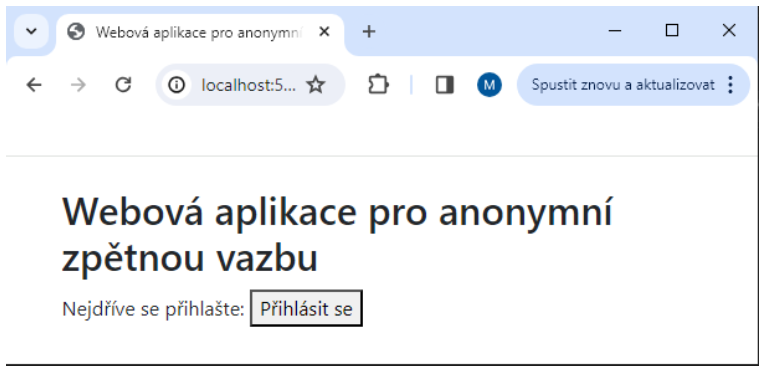
\includegraphics[width=0.7\textwidth]{login}
  \caption{login.html}
  \label{fig:obrazek}
\end{figure}


Aktivní otázky (myactive\_questions.html): Tento soubor je určen k zobrazení seznamu otázek, na které mohou studenti v danou chvíli odpovídat. Díky našemu backendu se zde každému studentovy zobrazují pouze otázky, které se ho týkají. U každé otázky jsou vypsané všechny informace, které student potřebuje znát, aby věděl na co přesně odpovídá. K jejich vypsání jsem využil: <label for="answer{{ question[0]}}"> <b>Akademický rok: </b> {{ question[3] }} Předmět: {{ question[4] }} Vyučující: {{ question[0] }} Otázka {{ question[1] }}</label>. Obsahuje formulář pro přidávání odpovědí a seznam zodpověditelných otázek. Formulář skládající se z libovolného počtu otázek, končí jediným tlačítkem, které uživateli umožní odpovědět na všechny otázky najednou.


\begin{figure}[h]
  \centering
  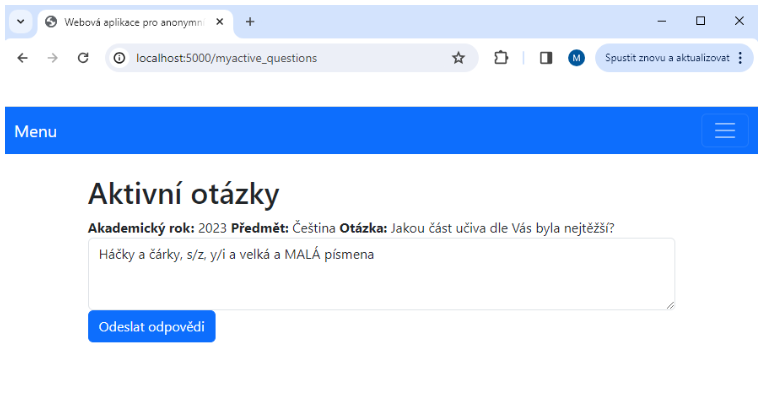
\includegraphics[width=0.7\textwidth]{myactivequestions}
  \caption{myactivequestions.html}
  \label{fig:obrazek}
\end{figure}

Přidání otázek (add\_question.html): Tento soubor slouží k přidávání nových otázek. Obsahuje dropdown komponentu pro výběr předmětu, ke kterému chce učitel zrovna přidat otázku a pole pro zadání nové otázky. Jednotliví vyučující zde také vidí seznam jimi přidaných otázek s tlačítkem smazat u každé z nich, aby se nikomu omylem nepodařilo smazat jinou otázku než zamýšlel. 

\begin{figure}[h]
  \centering
  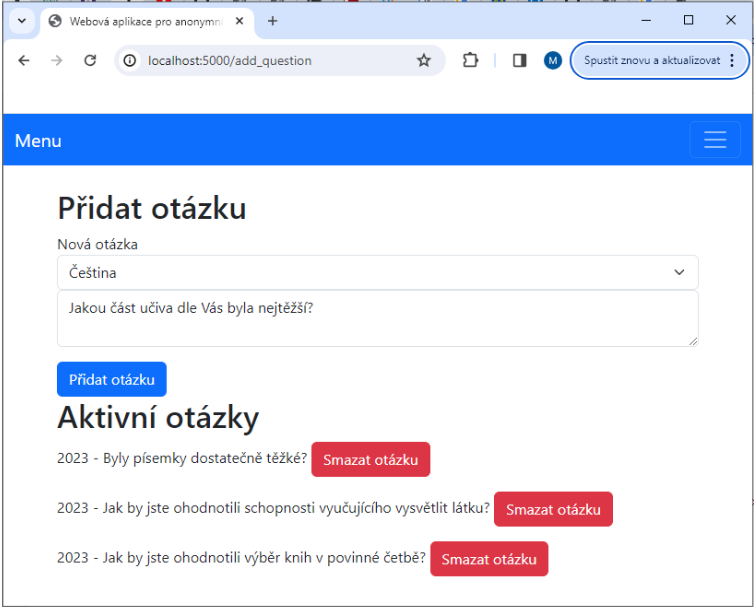
\includegraphics[width=0.7\textwidth]{addquestion}
  \caption{addquestion.html}
  \label{fig:obrazek}
\end{figure}

Historie odpovědí (myanswers.html): Tento soubor slouží k zobrazení historie odpovědí uživatelů na otázky napříč rokama. Umožňuje jak učitelům, tak studentům procházet všechny otázky sloužící jako linky pro zobrazení odpovědí. Ty jsou i tady seřazeny od nejnovějších po nejstarší. Obsahuje dropdown link pro výběr předmětu, ke kterému hledáte zpětnou vazbu. Třídění je úmyslně nezávisle na učitelích, to umožní zobrazit více otázek najednou, jejichž odpovědi pak můžeme

\begin{figure}[h]
  \centering
  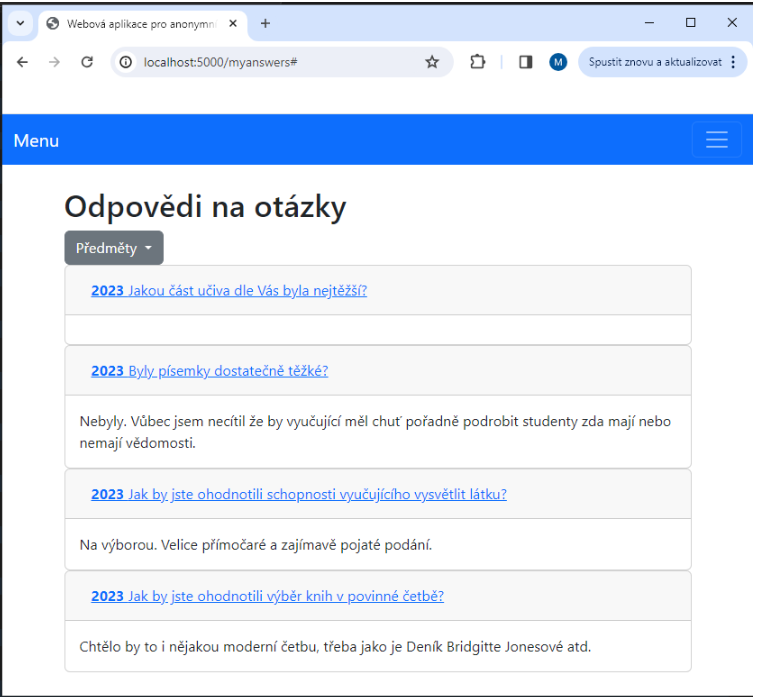
\includegraphics[width=0.7\textwidth]{myanswers}
  \caption{myanswers.html}
  \label{fig:obrazek}
\end{figure}

Soubor MyDbConnError.html je HTML stránka, která se zobrazí pouze pokud je problém s připojením do databáze.

\section{Bootstrap}

Integrace frameworku Bootstrap mi umožnila využít širokou škálu předdefinovaných komponent, jako jsou tlačítka, navigační panely, formulářové prvky a mnoho dalšího. Poskytl také responzivní mřížový systém, který umožnil naší aplikaci automaticky přizpůsobit se různým zařízením. Tyto komponenty jsem díky přehledné dokumentaci na stránkách vývojářů snadno integroval rovnou do našich HTML šablon pomocí jednoduchých kódů např.: <nav class="navbar navbar-expand-lg navbar-dark bg-primary"> což je element definující interaktivní hlavičku a její responzivní rozměry. Jednotlivé navigační položky se pak definují třídou(<li class="nav-item">). Pak už jen stačilo do hlavní souboru mybase.html přidat vývojářem poskytnuté odkazy.

\section{Jinja}
Jinja je šablonovací systém pro jazyk Python, který umožňuje vkládat dynamický obsah do statických šablon. Tento systém používán k generování dynamických HTML stránek. Jinja umožňuje vkládat proměnné, podmínky, smyčky a další konstrukce přímo do HTML šablon, což umožňuje tvorbu šablonových souborů s proměnlivým obsahem. Jinja šablony jsou vykreslovány serverem při požadavku na danou URL adresu. To umožňuje dynamicky generovat obsah stránky.

\chapter{BackEnd}

\section{Framework Python Flask}
Jako základ jsem zvolil Python Flask. Jedná se o webový framework napsaný v jazyce Python, který díky svých knihoven nabízí flexibilitu a snadnou použitelnost. Je známý pro svou jednoduchost a existuje na něj spousta tutoriálů. Jednotlivé knihovny se importují pomocí příkazu import a názvu modulu/knihovny mysql,connector, requests… V případě přidání vlastního modulu je potřeba nutno doplnit i adresu odkud přidáváme jako jsou blueprinty například takto: from auth import auth\_bp.

\section{MySQL}
Jako relační databázový systém pro správu dat používá aplikace MySQL. Byl zvolen protože jej lze využívat zdarma s licencí GPL a dá se velmi snadno nainstalovat a zprovoznit. Zároveň je to jeden z nejpoužívanějších databázových systému, díky čemuž obsahuje rozsáhlé dokumentace. Tento bod se zabývá návrhem a implementací databáze, včetně definice tabulek, vztahů mezi nimi a manipulace s daty. Struktura databáze obsahuje tabulky pro uchování informací o uživatelích, předmětech, otázkách a odpovědích. Propojení těchto tabulek pomocí cizích klíčů nám umožňuje implementovat do aplikace jednotlivé funkce potřebné pro získávání zpětné vazby. Prvním krokem pro implementaci databáze byl návrh tabulek.

\section{Implementace databáze}

Pro propojení webové aplikace s databází MySQL jsem využil knihovnu mysql.connector. Tato knihovna mi umožnila vytvořit spojení s databází pomocí konfiguračních údajů \{‘host’, ’user’, ’password’ a ’database’\}, které jsem uložil do proměnné DB\_CONFIG.
Poté jsem vytvořil funkci connect(), která se pokusí vytvořit spojení s databází pomocí mysql.connector.connect(**DB\_CONFIG). Pokud se spojení vytvoří úspěšně, funkce vrátí objekt spojení. Pokud dojde k chybě, funkce vrátí None.
Dále jsem vytvořil funkce insert\_data() a delete\_data(), které umožňují vkládání a mazání dat z databáze. Tyto funkce přijímají objekt spojení, SQL dotaz a data pro dotaz jako parametry. Využívají metodu execute() objektu cursor pro provedení SQL dotazu a metodu commit() objektu spojení pro uložení změn do databáze.
Konečně, jsem vytvořil funkci insert\_answer\_and\_student\_question, která využívá funkci insert\_data() pro vložení odpovědi a otázky studenta do databáze.

\section{Autentizace}

Pro autentizaci uživatelů jsem měl použít Google OAuth. Toto rozhodnutí zajišťuje bezpečnost a pohodlí uživatelů, kteří se tak mohou přihlásit pomocí svého stávajícího Google účtu.
Pro komunikaci s Google API a získání autorizačních toků jsem využil modul Requests. Nejprve jsem získal autentizační údaje pomocí flow.credentials a následně vytvořil session pro HTTP požadavky pomocí requests.session(). Tato session byla uložena do mezipaměti pomocí cachecontrol, což mi umožnilo omezit opakované požadavky na server.
Pro integraci OAuth autentizace byla použita knihovna Flask-OAuthlib. Po vytvoření projektu v Google Developers Console a získání autentizačních klíčů jsem definoval routy pro přihlášení a odhlášení uživatelů pomocí metod poskytovaných rozšířením Flask-OAuthlib.

\section{Tabulky}
Těch bylo potřeba osm. Musel jsem totiž zařídit, aby mohl každý učitel přidávat otázky pouze k předmětům, které učí a pouze v roce, kdy je učí. A aby každý student mohl zas odpovídat jen na otázky vztahující se ke konkrétním předmětům, které se učí. Pro snazší pochopení se dají rozdělit do tří skupin:
\subsection{Nezávislé:}
Do této kategorie patří tabulky students, teachers a subjects, nesoucí hlavní klíče o uživatelích a předmětech.
\subsection{Data zpětné vazby:}
Zde jsou tabulky questions a answers. Ty slouží pro správu uživateli přidaných dat jako jsou otázky, odpovědi a rok jejich přidání. Obě tabulky obsahují cizí klíče pro přizování otázek k učitelům a odpovědí k otázkám viz. diagram.
\subsection{Relace:}
Poslední tři tabulky vytváří relace potřebné pro správu dat. Patří mezi ně teacher\_subject, enrollments a student\_question.
Tabulka teacher\_subject:
Tato tabulka slouží k zachycení vztahu mezi vyučujícími a předměty. Slouží jako orientační bod v každé otázce. To znamená, že každý učitel má možnost pokládat otázky pouze na předměty které učí. Je to funkce nezbytná pro zachování pořádku ve zpětné vazbě.
Tabulka enrollments:
Tato tabulka slouží k evidenci, který student je zapsán na který předmět a od kterého učitele. Využívá k tomu cizí klíče student\_id a teacher\_subject\_id. To umožňuje správu studentských zápisů, jinými slovy to slouží k filtrování otázek na které může daný student odpovídat. A to v závislosti na tom jestli je a nebo není konkrétní student zapsán na kurzu, ke kterému byla otázka položena.
Tabulka student\_question:
Zaznamenává relace mezi studenty a otázkami, na které odpověděli. Je potřebná pro zajištění toho, aby mohl student odpovědět na každou otázku pouze jednou, přičemž by si zároveň zachoval anonymitu.
Většina dat se tedy bude muset do databáze doplňovat přímo.


\begin{figure}[h]
  \centering
  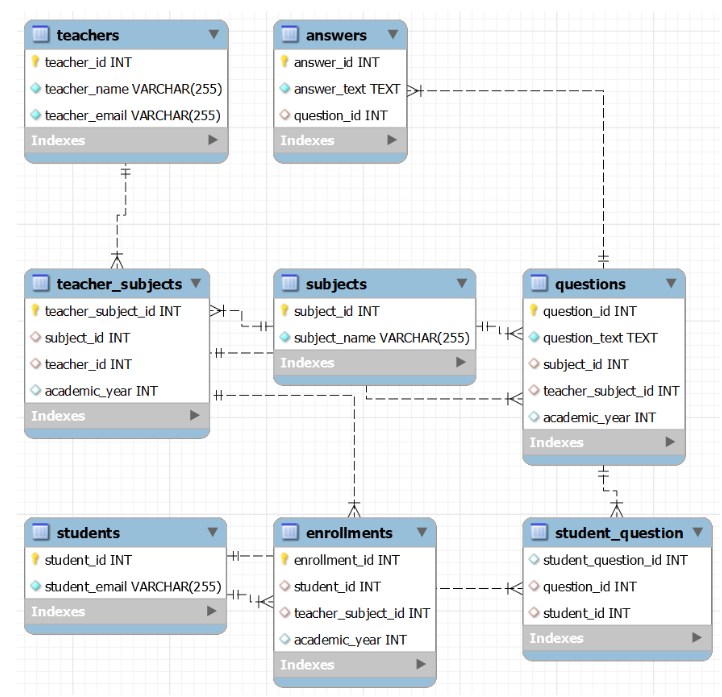
\includegraphics[width=0.8\textwidth]{database_structure}
  \caption{Databázový diagram}
  \label{fig:obrazek}
\end{figure}



\chapter*{Závěr}
\pagestyle{empty}
\addcontentsline{toc}{chapter}{Závěr}

Práce na tomto projektu pro mě byla něčím úplně novým. Přestože jsem se v tom ze začátku docela ztrácel a moc jsem netušil, co všechno budu muset udělat. Celkově si myslím, že se mi podařilo dosáhnout většiny cílů, které jsem měl. Aplikace umožňuje definovat otázky, sbírat odpovědi a analyzovat data z minulých let. Žáci mohou odpovídat pouze na otázky, které jsou jim určeny. Učitelé mají možnost otázky nejen přidávat ale i odebírat. To ale jen v případě, že na danou otázku ještě není přidaná jediná odpověď. To mi totiž přišlo jako objektivnější řešení pro získávání zpětné vazby, aby si učitelé nemohli mazat otázky obsahující kritiku. Teď zpětně ale přemýšlím, že by mělo vedení školy nějakou formu regulace obsahu mít. Jsem si samozřejmě vědom některých nedokonalostí, kterých jsem se ve svých řešení dopustil.
Asi největším prohřeškem bylo zařízení  anonymity pomocí databázové tabulky student\_question , které anonymitu zajišťuje pouze při větším množství odpovědí na danou otázku. Další nedokonalostí je určitě struktura mého kódu, který jsem mohl napsat lépe. Samotná práce pro mě bylo velkou zkušeností a doufám, že své nově nabité zkušenosti budu moci ještě někdy využít. Vlastně všechno, co jsem v projektu dělal až na psaní html kódů pro mě bylo novinkou. Od navrhování databáze až po implementaci jednotlivých funkcí v Python Flask. Také jsem se setkal s vývojem webových aplikací z hlediska autentizace uživatelů pomocí google oauth.

\chapter{Citace}

\section{}
Mark Otto, J. T. (n.d.). Introduction. Bootstrap.
 
https://getbootstrap.com/docs/4.1/getting-started/introduction/ 

\section{}
MySQL Workbench. MySQL. (n.d.). 

https://dev.mysql.com/doc/workbench/en/ 

\section{}
Welcome to flask. Welcome to Flask - Flask Documentation (3.0.x). (n.d.-a). 

https://flask.palletsprojects.com/en/3.0.x/ 

\section{}
GfG. (2023, December 1). Flask Tutorial. GeeksforGeeks. 

https://www.geeksforgeeks.org/flask-tutorial/ 

%%% Seznam použité literatury
%%%\cite{palletsprojects}\cite{flask-tutorial}\cite{Workbench}\cite{Bootstrap}
\printbibliography[title={Seznam použité literatury},heading={bibintoc}]

%%% Seznam obrázků
\openright
\listoffigures
\addcontentsline{toc}{chapter}{Seznam obrázků}

%%% Seznam tabulek
\clearpage
\listoftables
\addcontentsline{toc}{chapter}{Seznam tabulek}

%%% Přílohy k práci, existují-li. Každá příloha musí být alespoň jednou
%%% odkazována z vlastního textu práce. Přílohy se číslují.

%\part*{Přílohy}
%\appendix

\end{document}
